\begin{Solution}{1}
        The block diagram can be constructed by simply writing the pertinent equations one after the other and labeling the intermediate signals.  The full diagram should look something like Fig.\ \ref{fig.sol.poscon.blockdiagram}.
        \begin{figure}
        \centering
        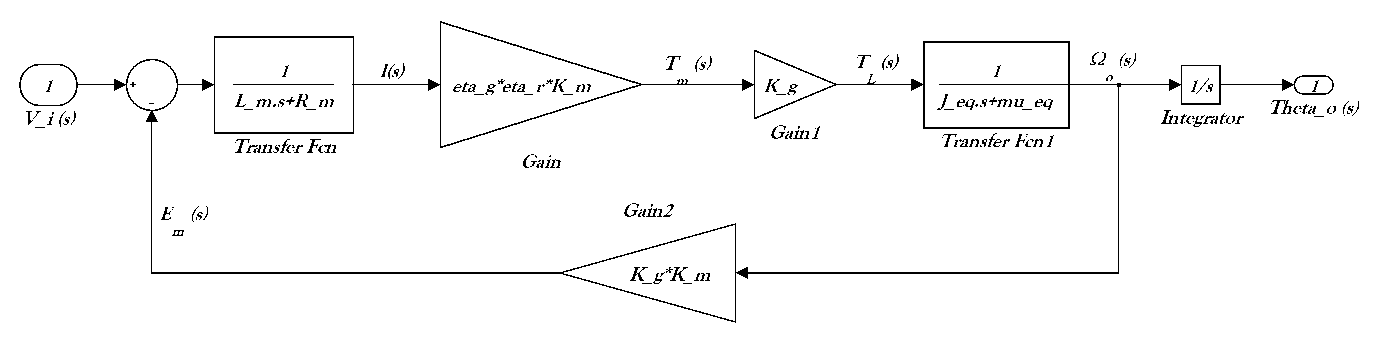
\includegraphics[angle=90, height=.95\textheight]{posconprelab1}
        \caption{\label{fig.sol.poscon.blockdiagram}}
        \end{figure}
        
\end{Solution}
\begin{Solution}{2}
        From the block diagram in question 1, it is a matter of reducing it to a single transfer function.  Use the rule that a negative feedback loop with block $G_1$ in the forward path and $G_2$ in the reverse path reduces to
        \begin{equation}
            G = \frac{G_1}{1+G_1G_2}
        \end{equation}
        After setting $L_m=0$, we have
        \begin{equation}
            TF_{V_i\to\Omega_o} =
                \frac{\frac{\eta K_m K_g}{R_m} \frac{1}{\mu_{eq} + J_{eq}s}}{ 1 + K_g K_m \frac{\eta K_m K_g}{R_m} \frac{1}{\mu_{eq} + J_{eq}s}}
        \end{equation}
        Note that $\eta := \eta_g \eta_r$.  To simplify, we multiply top and bottom of the big fraction by $\mu_{eq} + J_{eq}s$ to get
        \begin{equation}
            = \frac{
                    \frac{
                            \eta K_m K_g
                            }{
                            R_m
                            }
                    }{
                    \mu_{eq} + J_{eq}s + \frac{
                                                \eta K_m^2 K_g^2
                                                }{
                                                R_m
                                                }
                    }
        \end{equation}
        And now multiplying top and bottom by $1/J_{eq}$, we arrive at
        \begin{equation}
            = \frac{
                    \frac{
                            \eta K_m K_g
                            }{
                            R_m J_{eq}
                            }
                    }{
                    s + \frac{
                                \mu_{eq}
                                }{
                                J_{eq}
                                }
                    + \frac{
                            \eta K_m^2 K_g^2
                            }{
                            R_m J_{eq}
                            }
                    }
        \end{equation}
        Thus we have the correct form with pole-zero constants:
        \begin{subequations}
        \begin{gather}
            a = \frac{\eta K_m K_g}{R_m J_{eq}} \approx 288.3844\\
            b = \frac{\mu_{eq}}{J_{eq}} + \frac{\eta K_m^2 K_g^2}{R_m J_{eq}}
                \approx 40.4091
        \end{gather}
        \end{subequations}
        \par
        Finally, to get the TF to output position, we only need to pass the above TF through an integrator (it will have the same constants $a$ and $b$):
        \begin{equation}
            TF_{V_i\to\Theta_o} =
                \frac{a}{s(s+b)}
        \end{equation}
    
\end{Solution}
\begin{Solution}{3}
        The FVT looks like
        \begin{equation}
            \lim_{t\to\infty} \theta_o(t) = \lim_{s\to0}s\Theta_o(s)
        \end{equation}
        Applying this to our system, we have
        \begin{equation}
            \lim_{t\to\infty} \theta_o(t)
            =
            \lim_{s\to0} s \frac{1}{s} \frac{a}{s(s+b)} = \infty
        \end{equation}
        Some explanation:  The leading $s$ comes from the FVT itself.  The $1/s$ gives the systems response to a step input.  The rest of the expression is simply the transfer function to output position found in Question 2.
        
\end{Solution}
\begin{Solution}{4}
        The inner feedback loop (the derivative control) in Fig.\ \ref{fig.servoPD} can be reduced to
        \begin{equation}
            G_1(s) := \frac{
                            \frac{a}{s+b}
                            }{
                            1+K_D\frac{a}{s+b}
                            }
        \end{equation}
        Then in the forward path of the remaining diagram, we have $K_P G_1(s)/s$.  The remaining diagram is a simple unity feedback system:
        \begin{equation}
            TF_{\Theta_i\to\Theta_o} :=
            \frac{K_P G_1(s)/s}{1+K_P G_1(s)/s}
                \label{eq.servoPDtf}
        \end{equation}
        Simplifying Equation~(\ref{eq.servoPDtf}) yields the classical second-order transfer function:
        \begin{equation}
            TF_{\Theta_i\to\Theta_o} =
            \frac{
                K_P a
                }{
                s^2 + s(b+K_D a) + K_P a
                }
                \label{eq.servoPD}
        \end{equation}
        
\end{Solution}
\begin{Solution}{5}
        Comparing Eqs.\ (\ref{eq.secondordertf}) and (\ref{eq.servoPD}), we can conclude the following basic parameters:
        \begin{subequations}
        \begin{flalign}
        K &= 1 \\
        \omega_n &= \sqrt{K_P a} \\
        \zeta &= \frac{b+K_D a}{2\sqrt{K_P a}} \label{eq.servoDR}
        \end{flalign}
        \end{subequations}
        We then translate the formula given for peak time into one with our parameters:
        \begin{equation}
        t_p =  \frac{\pi}{\omega_n \sqrt{1-\zeta^2}}
        = \frac{
                \pi
                }{
                \sqrt{K_P a}\sqrt{1-\frac{
                                        (b+K_D a)^2
                                        }{
                                        4K_P a
                                        }
                                        }
                }
            \label{eq.servoPT}
        \end{equation}
        Now we have a system of equations with two unknowns ($K_P$, and $K_D$) and two equations (\ref{eq.servoDR} and \ref{eq.servoPT}).  You can solve these using your favorite method.  One way would be to rearrange Eq.\ \ref{eq.servoDR} for $K_D$ and then substitute into Eq.\ \ref{eq.servoPT} to solve for $K_P$ first.  Using $K_P$, you can then go back and find $K_D$.
        \par
        These parameters turn out to be:
        \begin{flalign*}
            K_P &\approx 27.3708 \\
            K_D &\approx 0.2955
        \end{flalign*}
        
\end{Solution}
\begin{Solution}{6}
        The solution to this question is provided in Fig.\ \ref{fig.servoPDmodel}.
        
\end{Solution}
